\pagebreak
\subsection{Tecnologie di supporto allo sviluppo}
\label{sez:tecnologie-supporto-sviluppo}

\subsubsection{\gls{npm}}

È il gestore ufficiale dei pacchetti per \textit{Node.js}, utilizzato per installare, condividere e gestire librerie e moduli \textit{JavaScript}. 
Facilita la configurazione e la gestione delle dipendenze nei progetti, rendendo lo sviluppo più efficiente.

\subsubsection{Docker}

Piattaforma che consente di creare e gestire applicazioni in \gls{container} leggeri e portatili.
I \gls{container} permettono l’isolazione delle applicazioni e delle loro dipendenze, garantendo consistenza tra ambienti di sviluppo, \textit{test} e produzione.\\
Sono altamente utilizzati nell'attuale panorama dello sviluppo \textit{software} per semplificare il \textit{deployment} e garantire la portabilità delle applicazioni.

\subsubsection{Postman}

Strumento che permette di testare in modo semplice le \gls{api}. 
Consente di inviare richieste \gls{http} ed analizzare le risposte andando a semplificare lo sviluppo ed il \textit{debugging} delle \gls{api}. \\
In {\hyperref[fig:postman]{Figura 1.7}} è possibile vedere un esempio di utilizzo di \textit{Postman} per effettuare una chiamata all'\gls{api} per
la generazione di un progetto, completa dei parametri necessari.

\begin{figure}[H]
    \label{fig:postman}
    \centering
    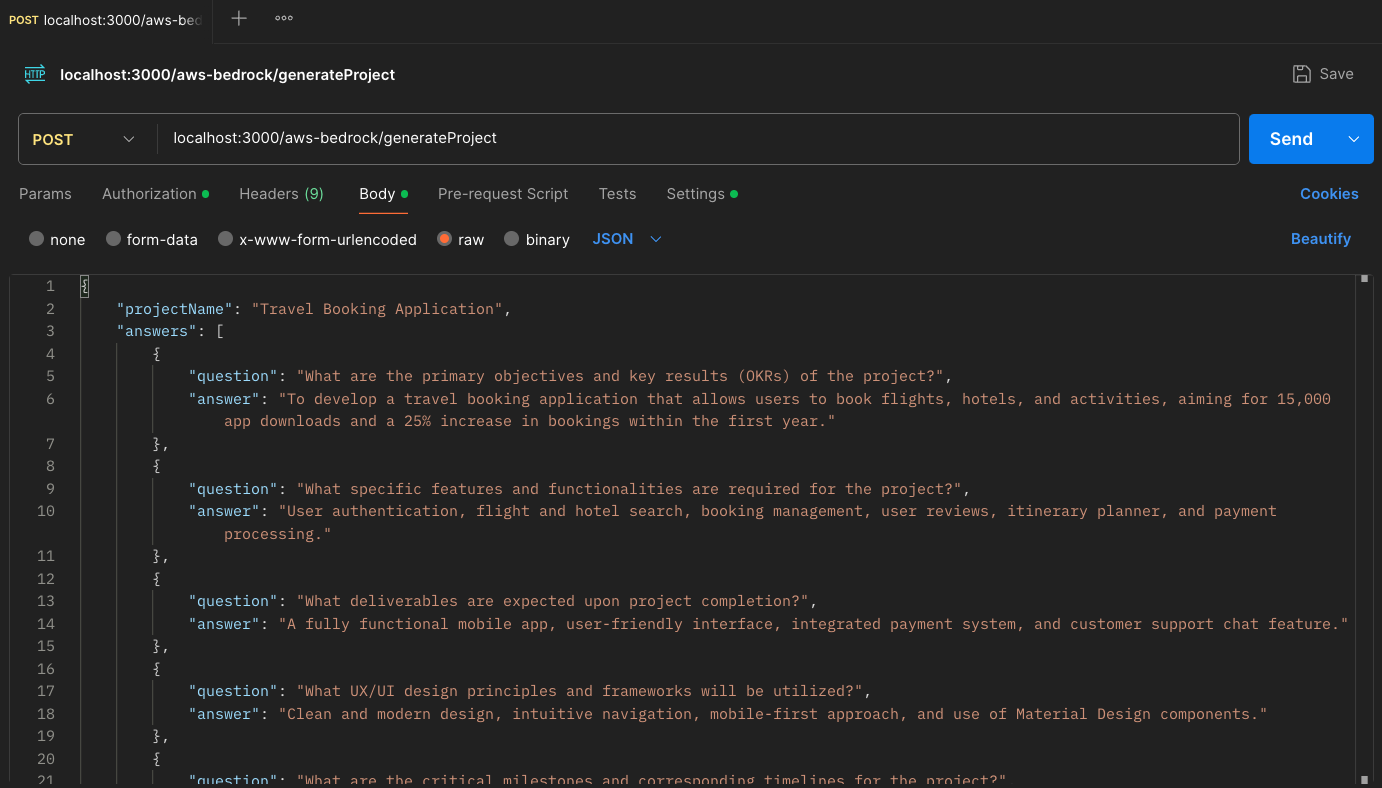
\includegraphics[scale=0.2]{tecnologie/postman.png}
    \caption{Esempio di utilizzo di \textit{Postman} per chiamata \gls{api}}
\end{figure}

\subsubsection{StarUML}

Uno strumento avanzato per la modellazione di \gls{uml}, utilizzato per creare e gestire diagrammi di progettazione software. Supporta un'ampia gamma di diagrammi \gls{uml}, tra cui casi d'uso, sequenza e attività, semplificando la visualizzazione di architetture e flussi.\\
I diagrammi \gls{uml} sono utilizzati per rappresentare in modo chiaro e conciso le relazioni tra i componenti di un sistema, facilitando la comprensione e la comunicazione tra gli sviluppatori, essendo un linguaggio altamente standardizzato.\\
\textit{StarUML} è stato utilizzato per creare i diagrammi dei casi d’uso del progetto.

\pagebreak
\subsubsection{git}

Un sistema di controllo di versione distribuito, progettato per tracciare le modifiche al codice sorgente e facilitare la collaborazione tra sviluppatori. \\
Permette di gestire versioni, ramificare progetti tramite l'utilizzo di \gls{branch} e integrare le modifiche in modo efficiente e sicuro. 

\subsubsection{MongoDB Compass}

Un'interfaccia grafica intuitiva per interagire con \textit{database MongoDB}, che consente di esplorare e modificare i dati, visualizzare indici e \textit{query},
e semplificare la gestione e l'analisi del \textit{database.}
Nella {\hyperref[fig:mongodb-compass]{Figura 1.8}} è possibile vedere un esempio di utilizzo di \textit{MongoDB Compass} per visualizzare un documento all'interno di una collezione.

\begin{figure}[H]
    \label{fig:mongodb-compass}
    \centering
    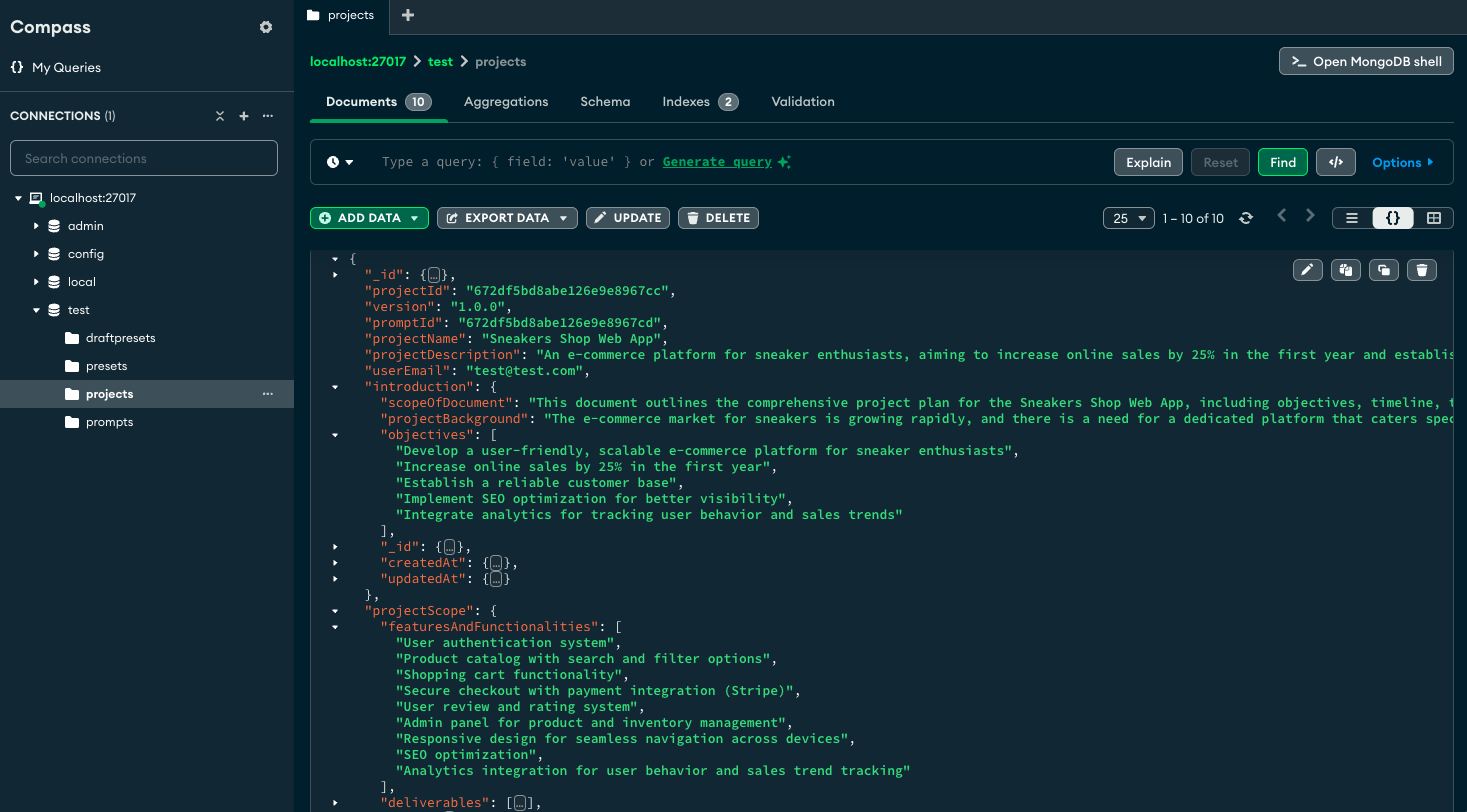
\includegraphics[scale=0.2]{tecnologie/mongodb-compass.png}
    \caption{Visualizzazione di un documento in \textit{MongoDB Compass}}
\end{figure}
